\documentclass[12pt,compress,aspectratio=169]{beamer}

\usetheme{metropolis}
\setbeamersize{text margin left=.5cm,text margin right=.5cm}
%\setbeamertemplate{navigation symbols}{} % suppress nav bar
%\setbeamercovered{transparent}

\usefonttheme{professionalfonts}
\usepackage{amsmath,bm}
\usepackage{siunitx}
\usepackage{tikz}
\usepackage{mathpazo}
%\usepackage[scaled]{helvet}
\usepackage{xcolor,colortbl}

\setmonofont{Ubuntu Mono}
\setlength{\parskip}{0pt}
\renewcommand{\baselinestretch}{1}

\sisetup{
  number-math-rm=\mathnormal,
  per-mode=symbol
}

\usetikzlibrary{decorations.pathmorphing,patterns}


\title{Topic 3: Work and Energy}
\subtitle{Advanced Placement Physics C}
\author[TML]{Dr.\ Timothy Leung}
\institute{Olympiads School}
\date{July 13, 2020}

\newcommand{\pic}[2]{\includegraphics[width=#1\textwidth]{#2}}
\newcommand{\mb}[1]{\ensuremath\mathbf{#1}}
\newcommand{\eq}[2]{\vspace{#1}{\Large\begin{displaymath}#2\end{displaymath}}}

\begin{document}

\begin{frame}
  \maketitle
\end{frame}

\begin{frame}{Files for You to Download}
  These are the slides and homework questions for this week.
  \begin{itemize}
  \item\texttt{PhysAP-03-workEnergy.pdf}--This week's slides on work and
    energy
    %\item\texttt{PhysAP-03-momentumImpulse.pdf}--Next week's slides on momentum,
      %impulse and general collisions.
  \item\texttt{PhysAP-03-Homework.pdf}--Homework problems for this topic.
  \end{itemize}
  Please download/print the PDF file before class. There is no advantage to
  copying notes that are already printed out for you. Instead, focus on details
  that aren't necessarily on the slides. If you want to print the slides, we
  recommend that you print 4 slides per page to save paper.
\end{frame}



\begin{frame}{Work and Energy}
  We start with some definition at are (unfortunately) not very useful:
  \begin{itemize}
    \item \textbf{Energy} is the ability to do work.
    \item \textbf{Work} is the mechanism in which energy is transformed.
  \end{itemize}
  Luckily, we can also use equations to define these concepts.
\end{frame}


\section{Work}

\begin{frame}{Work}
  \textbf{Mechanical work} $dW$ is performed when a force $\mb{F}$ is used to
  displace an object by an infinitesimal amount $d\mb{x}$. If a varying force
  is applied to move an object from $\mb{x}_1$ to $\mb{x}_2$ along a path, then
  the total work done by the force is defined by the integral:

  \eq{-.25in}{
    W=\int\mb{F}(\mb{x})\cdot d\mb{x}
  }

  \begin{itemize}
  \item No work done if the force is perpendicular to displacement
    (i.e.\ $\mb{F}\cdot d\mb{x}=0$)
  \item No work done if no displacement ($d\mb{x}=\mb{0}$)
  \item Work can be positive or negative depending on the dot product
  \item When there are multiple forces acting on an object, we can compute the
    work done by each \emph{each} force
  \end{itemize}
\end{frame}



\begin{frame}{Work by Constant Force}
  For a constant force, if the object moves along straight path, the integral
  simplifies to just the dot product of the two vectors:

  \eq{-.2in}{
    W=\mb{F}\cdot\Delta\mb{r}
  }

  Or in the scalar form that is more familiar in Grades 11/12 Physics that
  avoid vector notations:

  \eq{-.2in}{
    \boxed{W=F\Delta x\cos\theta}
  }

  \vspace{-.1in}where $\theta$ is the angle between the force and displacement
  vectors
\end{frame}



\begin{frame}{Definition of Work}
  \textbf{Work done by a force}
  \begin{itemize}
  \item The work done by \emph{one specific force}
  \item Example: A boy pushes a cart forward. The ``work done by the boy'' is
    the work done by the applied force.
  \end{itemize}

  \vspace{.15in}\textbf{Work done on an object}
  \begin{itemize}
  \item There may be more than one force acting on an object
  \item The \emph{sum} of all the work done on the object by each force
  \item The work done by the net force
  \item Also called the \textbf{net work} $W_\mathrm{net}$
  \end{itemize}
\end{frame}


\section{Kinetic Energy}

\begin{frame}{Kinetic Energy}
  When a net force on an object accelerates it, the resulting amount of
  work done on the object (net work $W_{\textrm{net}}$) is given by:

  \eq{-.2in}{
    W_{\textrm{net}}=\int\mb{F}_{\textrm{net}}\cdot d\mb{x}=\int m\mb{a}\cdot d\mb{x}
    =m\int\frac{d\mb{v}}{dt}\cdot d\mb{x}
  }

  Since both $\mb{v}$ and $\mb{x}$ are continuous functions in
  time, we can switch the order of differentiation, i.e.:

  \eq{-.2in}{
    =m\int\frac{d\mb{x}}{dt}\cdot d\mb{v}=m\int\mb{v}\cdot d\mb{v}
    =m\int_{v_1}^{v_2} vdv %=\Delta\left(\frac{1}{2}mv^2\right)=\Delta K
  }

  and since $\mb{v}$ and $d\mb{v}$ must be in the same direction, the dot
  product is trivial: $\mb{v}\cdot d\mb{v}=vdv$
\end{frame}



\begin{frame}{Kinetic Energy}
  This integral, when integrated from $v_1$ (initial speed) to $v_2$
  (final speed), becomes:

  \eq{-.2in}{
    =m\int_{v_1}^{v_2} vdv=\frac{1}{2}mv^2\Big|^{v_2}_{v_1}=\Delta K
  }
  
  where $K$ is defined as the \textbf{translational kinetic energy}:

  \eq{-.1in}{
    K=\frac12mv^2
  }
\end{frame}



\begin{frame}{Work and Kinetic Energy}
  In fact, the \emph{definition} of kinetic energy came from this integration,
  in that, work equals to the change in \emph{something}, and we define that as
  kinetic energy. This is the \textbf{work-energy theorem}:

  \eq{-.15in}{
    W_\mathrm{net}=\Delta K
  }
  \begin{itemize}
  \item\vspace{-.15in} $\Delta K$ can be positive or negative depending on the
    dot product
  \item There may be multiple forces acting on an object; each of the forces
    can add or take away kinetic energy from an object
  \item Therefore we use the ``net'' amount of work done in the above equation
  \end{itemize}
\end{frame}



\begin{frame}{Example}
  \textbf{Example 1:} A force $\mb{F}=4.0x\bm{\hat{\imath}}$ (in newtons) acts
  on an object of mass \SI{2.}{\kilo\gram} as it moves from $x=1.0$ to
  $x=\SI{5.}{\metre}$. Given that the object is at rest at $x=1$,
  \begin{enumerate}[(a)]
  \item Calculate the net work
  \item What is the final speed of the object?
  \end{enumerate}
\end{frame}



\section{Potential Energy}

\begin{frame}{Gravitational Force \& Potential Energy}
  The gravitational force (weight) of an object is defined as:
  
  \eq{-.25in}{
    \mb{w}=m\mb{g}
  }
  
  \vspace{-.1in}For objects near the surface of Earth, we assume that
  $\mb{g}=-g\bm{\hat{\jmath}}=-9.81\bm{\hat{\jmath}}$ (in
  \si{\metre\per\second^2}) is constant. The work done to move an object
  from height $h_1$ to $h_2$ is therefore:

  \eq{-.2in}{
    W=\int \mb{w}\cdot d\mb{h}
    =\int_{h_1}^{h_2} -mg\bm{\hat{\jmath}}\cdot dh\hat{\bm{\jmath}}
    =-mgh\Big|^{h_2}_{h_1}=-\Delta U_g
  }

  where $U_g$ is the \textbf{gravitational potential energy}:

  \eq{-.2in}{
    U_g=mgh
  }
\end{frame}




\begin{frame}{Spring Force \& Elastic Potential Energy}
  The spring force $\mb{F}_e$ is the force a compressed or stretched spring
  exerts onto objects connected to it. It obeys Hooke's law:
    
  \eq{-.2in}{
    \mb{F}_e=-k\mb{x}
  }

  \vspace{-.1in}We can find the work done to displace a spring:

  \eq{-.3in}{
    W=\int\mb{F}_e\cdot d\mb{x}=-k\int xdx=-\frac{1}{2}kx^2\Big|^{x_2}_{x_1}
    =-\Delta U_e
  }
  
  where $U_e$ is the \textbf{elastic potential energy}:

  \eq{-.2in}{
    U_e=\frac12kx^2
  }
\end{frame}



\begin{frame}{Conservative Forces}
  Gravitational force, spring force, electrostatic force (later in the
  course) are called \textbf{conservative forces}
  \begin{itemize}
  \item The work done by these forces relate to a change of another quantity
    called \emph{potential energy}
  \item Since the potential energy is evaluated at the end points, the work
    done by a conservative force is \emph{path independent}
  \end{itemize}
\end{frame}



\begin{frame}{Conservative Forces}
%  \begin{itemize}
%  \item Gravitational force, spring force,  electrostatic force (later in the
%    course) are called \textbf{conservative forces}
%  \item Work done by a conservative force is independent of the path taken
  Expressions for potential energies are obtained by integrating the work done
  by the conservative forces, these forces are therefore the negative gradient
  of the potential energies:

  \eq{-.2in}{
    \mb{F}=-\nabla U=
    -\frac{\partial U}{\partial x}\bm{\hat{\imath}}
    -\frac{\partial U}{\partial y}\bm{\hat{\jmath}}
    -\frac{\partial U}{\partial z}\hat{\bm{k}}
  }

  The direction of a conservative force \emph{always} decreases the potential
  energy. In 1D:

  \eq{-.2in}{
    \mb{F}=-\frac{dU}{dx}
  }

  Pay attention to the negative sign. Students often forget it.
\end{frame}




\begin{frame}{Work and Potential Energy}
  The expressions for potential energies also come from integrating the work
  equation, in that work equals to the change in \emph{something}, and we
  called that potential energy. Therefore:

  \eq{-.2in}{
    W=-\Delta U
  }
  \begin{itemize}
  \item\vspace{-.15in}$\Delta U$ can be positive or negative depending on the
    direction of the (conservative) force
  \item Positive work \emph{decreases} the related potential energy
  \item Negative work \emph{increases} the related potential energy
  \end{itemize}
\end{frame}



\begin{frame}{Conservation of Mechanical Energy}
  Positive work done by conservative forces on an object does two things:
  \begin{enumerate}[1.]
  \item Decrease its potential energy, while
  \item Increase its kinetic energy by the same amount
  \end{enumerate}
  Mathematically, this shows that mechanical energy must always be conserved
  when there are only conservative forces:

  \eq{-.15in}{
    W=-\Delta U = \Delta K \quad\longrightarrow\quad
    \Delta K + \Delta U =0
  }

  That's why those forces are called conservative forces!
\end{frame}



\section{Conservation of Energy}

\begin{frame}{Isolated Systems and the Conservation of Energy}
  An \textbf{isolated system} is a system of objects that does not interact with
  the surrounding. Think of an isolated system as a bunch of objects inside an
  insulated box.
  \begin{center}
    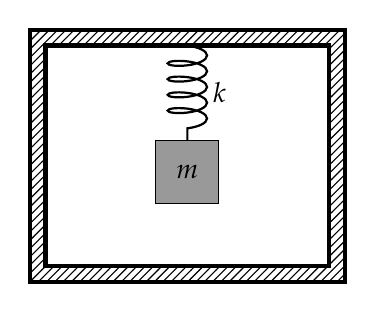
\begin{tikzpicture}[scale=.8]
      \fill[pattern=north east lines] (0,0) rectangle(5,4);
      \draw[ultra thick] (0,0) rectangle(5,4);
      \draw[ultra thick,fill=white](.25,.25) rectangle(4.75,3.75);
      \draw[thick,
        decoration={aspect=.3,segment length=2mm, amplitude=2.5mm, coil},
        decorate] (2.5,3.75)--(2.5,2.25) node[midway,right]{$\;\;k$};
      \draw[fill=black!40](2,2.25) rectangle(3,1.25) node[midway]{$m$};
    \end{tikzpicture}
  \end{center}
\end{frame}


\begin{frame}{Isolated Systems and Conservation of Energy}
  \begin{itemize}
  \item Since the system is isolated from the surrounding environment, the
    environment can't do any work on it, by definition!
  \item Likewise, the energy inside the system cannot escape either
  \item Therefore energy of the system is conserved
  \item There are \emph{internal} force inside the system that is doing work,
    but the work only converts kinetic energy into potential energies, and vice
    versa.
  \end{itemize}
\end{frame}



\begin{frame}{Example: Mass sliding on a spring}
  \begin{itemize}
  \item Assuming that there is no friction in any part of the system
  \item The isolated system consists of the mass and the spring 
  \item Energies:
    \begin{itemize}
    \item Kinetic energy of the mass
    \item Elastic potential energy stored in the spring
    \end{itemize}
  \end{itemize}
  \begin{center}
    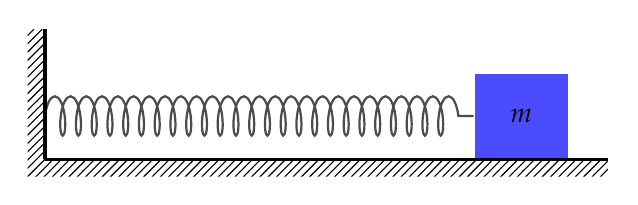
\begin{tikzpicture}[scale=1.1]
      \node[fill=blue!70,inner sep=4.5mm] (a) at (5.5,1) {$m$};
      \draw[thick,draw=black!70,
        decoration={aspect=.3,segment length=2mm, amplitude=2.5mm, coil},
        decorate] (0,1)--(4.95,1);
      \fill [pattern=north east lines] (6.5,.5)--(6.5,.3)--(-.2,.3)
      --(-.2,2)--(0,2)--(0,.5)--cycle;
      \draw[very thick] (0,.5)--(6.5,.5);
      \draw[very thick] (0,.5)--(0,2);
    \end{tikzpicture}
  \end{center}
\end{frame}


\begin{frame}{Example: Gravity}
  \begin{center}
    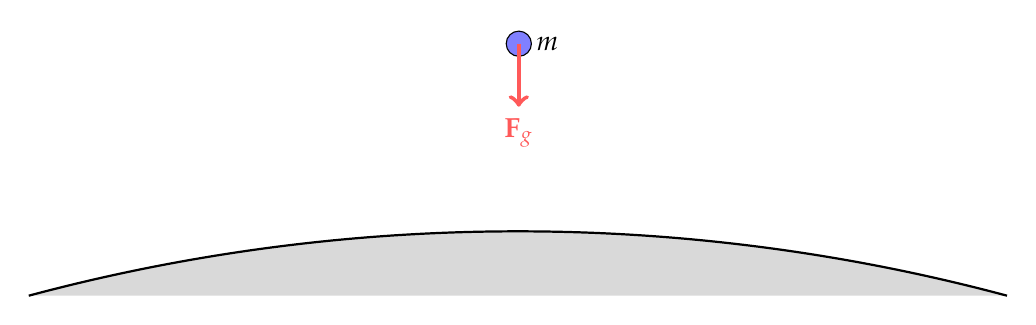
\begin{tikzpicture}[scale=.8]
      \draw[thick,fill=gray!30] (7.75,0) arc(75:105:30);
      \draw[fill=blue!50] (0,4) circle(.2) node[right]{$\;m$};
      \draw[ultra thick, red!65,->] (0,4)--(0,3) node[pos=1,below]{$\mb{F}_g$};
    \end{tikzpicture}
  \end{center}
  
  \begin{itemize}
  \item The isolated system consists of the mass and Earth
  \item Assuming no friction
  \item Energies:
    \begin{itemize}
    \item Kinetic energy of the mass
    \item Gravitational potential energy of the mass
    \end{itemize}
  \end{itemize}
\end{frame}



\begin{frame}{Example: Vertical spring-mass system}
  \begin{columns}
    \column{.17\textwidth}
    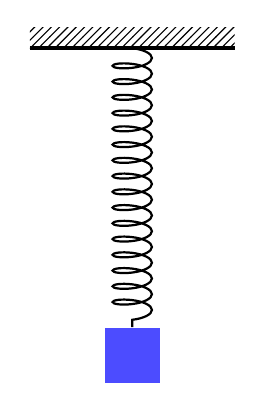
\begin{tikzpicture}[scale=1.3]
      \node[fill=blue!70,inner sep=3.5mm] (b) at (1,2) {};
      \draw[thick,
        decoration={aspect=.3,segment length=2mm, amplitude=2.5mm, coil},
        decorate] (1,5)--(b); 
      \fill [pattern=north east lines] (0,5) rectangle (2,5.2);
      \draw[ultra thick] (0,5)--(2,5);
    \end{tikzpicture}
    \column{.85\textwidth}
    \begin{itemize}
    \item The system consists of a mass, a spring and Earth
    \item Energies:
      \begin{itemize}
      \item Kinetic energy of the mass
      \item Gravitational potential energy of the mass
      \item Elastic potential energy stored in the spring
      \end{itemize}
    \item The total energy of the system is conserved if there is no friction
    \end{itemize}
  \end{columns}
\end{frame}



\begin{frame}{What if there is friction?}
  Energy is always conserved as long as your system is defined properly
  \begin{columns}
    \column{.2\textwidth}
    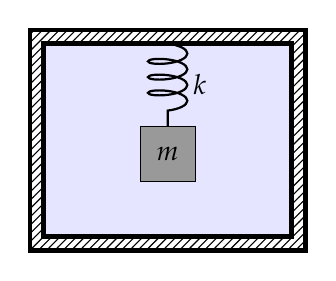
\begin{tikzpicture}[scale=.7]
      \fill[pattern=north east lines] (0,0) rectangle(5,4);
      \draw[ultra thick] (0,0) rectangle(5,4);
      \draw[ultra thick,fill=blue!10](.25,.25) rectangle(4.75,3.75);
      \draw[thick,
        decoration={aspect=.3,segment length=2mm, amplitude=2.5mm, coil},
        decorate] (2.5,3.75)--(2.5,2.25) node[midway,right]{$\;\;k$};
      \draw[fill=black!40](2,2.25) rectangle(3,1.25) node[midway]{$m$};
    \end{tikzpicture}
    \column{.8\textwidth}
    \begin{itemize}
    \item The system consists of a mass, a spring, Earth and all the air
      particles inside the box
    \item As the mass vibrates, friction with air slows it down
    \item While the mass loses energy, the temperature of the air rises due to
      friction
    \item Energies:
      \begin{itemize}
      \item Kinetic and gravitational potential energies of the mass
      \item Elastic potential energy stored in the spring
      \item Kinetic energy of the vibration of the air molecules
      \end{itemize}
    \item Total energy is conserved even as the mass stops moving
    \end{itemize}
  \end{columns}
\end{frame}



\begin{frame}{Conservation of Energy}
  If there are only conservative forces, mechanical energy (i.e.\ $K+U$) is
  always conserved:

  \eq{-.2in}{
    \boxed{K +U =K'+U'}
  }
  
  When non-conservative forces are also doing work, instead of
  \emph{trying} to isolate the system, we can calculate the work done by them
  $W_{\textrm{nc}}$ and add it to the total energy of the system
    
  \eq{-.2in}{
    \boxed{K+U+W_{\textrm{nc}}=K'+U'}
  }
\end{frame}



\begin{frame}{Work By Non-Conservative Force}
  Examples of non-conservative forces include:
  \begin{itemize}
  \item Work done by these forces are \emph{usually} negative because they
    oppose the direction of motion
    \begin{itemize}
    \item Drag (fluid resistance)
    \item Kinetic friction
    \end{itemize}
  \item The work done by these forces may be positive or negative, depending on
    the problem
    \begin{itemize}
    \item Applied force
    \item Tension force
    \item Normal force
    \end{itemize}
  \end{itemize}
  Note that the work-kinetic energy theorem still applies when non-conservative
  forces are present
\end{frame}


\begin{frame}{Example}
  \textbf{Example 2:} A mass $m$ is dropped from a height of $h$ above the
  equilibrium position of a spring. Set up the equation that determines the
  spring's compression $d$ when the object is instantaneously at rest.
  \begin{center}
    \pic{.35}{spring-example1.png}
  \end{center}
\end{frame}


%\begin{frame}{Example}
%  \textbf{Example 3:} A mass $m$ is pulled a distance $d$ up an incline (angle
%  of elevation $\theta$) at constant speed using a rope that is parallel to
%  the incline. The coefficient of friction is $\mu_k$.
%  \begin{enumerate}[(a)]
%  \item What is the magnitude of the tension force in the rope?
%  \item What is the magnitude of the normal force?
%  \item What is the work done by the normal force?
%  \item What is the work done by friction?
%  \item What is the work done by the tension force?
%  \item What is the net work?
%  \item What is the change in total mechanical energy?
%  \item Show that $\Delta E_\mathrm{mech}=W_\mathrm{non-conservative}$.
%  \end{enumerate}
%\end{frame}


\begin{frame}{Energy Diagrams}
  \begin{itemize}
  \item Plots of potential energy ($U$) vs.\ position for a conservative force
    \begin{center}
      \pic{.5}{energy-diagram.png}
    \end{center}
  \item If more than one conservative force, they can be combined into one graph
  \item Where slope is zero means no force acting on it: it is in a state of
    \textbf{equilibrium}
  \item An object placed at an equilibrium point with $K=0$ will remain there
  \end{itemize}
\end{frame}


\section{Power \& Efficiency}

\begin{frame}{Power}
  \textbf{Power} is the \emph{rate} at which work is done, i.e.\ the rate at
  which energy is being transformed:

  \eq{-.2in}{
    \boxed{P = \frac{dW}{dt}}\quad\quad
    \boxed{\bar{P} = \frac{W}{\Delta t}}
  }
  \begin{center}
    \begin{tabular}{l|c|c}
      \rowcolor{pink}
      \textbf{Quantity}  & \textbf{Symbol} & \textbf{SI Unit} \\ \hline
      Instantaneous and average power & $P$, $\bar{P}$ & \si{\watt} \\
      Work done          & $W$ & \si{\joule} \\
      Time interval      & $\Delta t$ & \si{\second}
    \end{tabular}
  \end{center}
  In engineering, power is often more critical than the actual amount of work
  done.
\end{frame}



\begin{frame}{Power}
  If a constant force is used to push an object at a constant velocity, the
  power produced by the force is:
  
  \eq{-.2in}{
    P=\frac{dW}{dt}=\frac{\mb{F}\cdot d\mb{x}}{dt}
    =\mb{F}\cdot\frac{d\mb{x}}{dt}
    \quad\rightarrow\quad
    \boxed{P=\mb{F}\cdot\mb{v}}
  }
  
  Application: aerodynamics
  \begin{itemize}
  \item When an object moves through air, the applied force must overcome air
    resistance (drag force), which is proportional with $v^2$
    \item Therefore ``aerodynamic power'' must scale with $v^3$ (i.e.\ doubling
      your speed requires $2^3=8$ times more power)
    \item Important when aerodynamic forces dominate
  \end{itemize}
\end{frame}



\begin{frame}{Efficiency}
  \textbf{Effieiency} is the ratio of useful energy or work output to the total
  energy or work input

  \eq{-.2in}{
    \eta = \frac{E_o}{E_i}\times\SI{100}{\percent}\quad
    \eta = \frac{W_o}{W_i}\times\SI{100}{\percent}
  }
  \begin{center}
    \begin{tabular}{l|c|c}
      \rowcolor{pink}
      \textbf{Quantity} & \textbf{Symbol} & \textbf{SI Unit} \\ \hline
      Useful output energy & $E_o$ & \si{\joule} \\
      Input energy         & $E_i$ & \si{\joule} \\
      Useful output work   & $W_o$ & \si{\joule} \\
      Input work           & $W_i$ & \si{\joule} \\
      Efficiency           & $\eta$ & no units
    \end{tabular}
  \end{center}
  Efficiency is always $0\leq\eta\leq\SI{100}{\percent}$
\end{frame}
\end{document}
